%% BioMed_Central_Tex_Template_v1.06
%%                                      %
%  bmc_article.tex            ver: 1.06 %
%                                       %

%%IMPORTANT: do not delete the first line of this template
%%It must be present to enable the BMC Submission system to
%%recognise this template!!

%%%%%%%%%%%%%%%%%%%%%%%%%%%%%%%%%%%%%%%%%
%%                                     %%
%%  LaTeX template for BioMed Central  %%
%%     journal article submissions     %%
%%                                     %%
%%          <8 June 2012>              %%
%%                                     %%
%%                                     %%
%%%%%%%%%%%%%%%%%%%%%%%%%%%%%%%%%%%%%%%%%


%%%%%%%%%%%%%%%%%%%%%%%%%%%%%%%%%%%%%%%%%%%%%%%%%%%%%%%%%%%%%%%%%%%%%
%%                                                                 %%
%% For instructions on how to fill out this Tex template           %%
%% document please refer to Readme.html and the instructions for   %%
%% authors page on the biomed central website                      %%
%% http://www.biomedcentral.com/info/authors/                      %%
%%                                                                 %%
%% Please do not use \input{...} to include other tex files.       %%
%% Submit your LaTeX manuscript as one .tex document.              %%
%%                                                                 %%
%% All additional figures and files should be attached             %%
%% separately and not embedded in the \TeX\ document itself.       %%
%%                                                                 %%
%% BioMed Central currently use the MikTex distribution of         %%
%% TeX for Windows) of TeX and LaTeX.  This is available from      %%
%% http://www.miktex.org                                           %%
%%                                                                 %%
%%%%%%%%%%%%%%%%%%%%%%%%%%%%%%%%%%%%%%%%%%%%%%%%%%%%%%%%%%%%%%%%%%%%%

%%% additional documentclass options:
%  [doublespacing]
%  [linenumbers]   - put the line numbers on margins

%%% loading packages, author definitions

\documentclass[twocolumn, notitlepage]{bmcart}% uncomment this for twocolumn layout and comment line below
%\documentclass{bmcart}

%%% Load packages
%\usepackage{amsthm,amsmath}
%\RequirePackage{natbib}
%\RequirePackage[authoryear]{natbib}% uncomment this for author-year bibliography
%\RequirePackage{hyperref}
\usepackage[utf8]{inputenc} %unicode support
%\usepackage[applemac]{inputenc} %applemac support if unicode package fails
%\usepackage[latin1]{inputenc} %UNIX support if unicode package fails

%*** para suportar tabelas com colunas mergeadas ***
\usepackage{multirow}
\usepackage[export]{adjustbox}



%*** Para inclusão de imagens e permitir rotacionar texto ***
\usepackage{graphicx}			% Inclusão de gráficos
\graphicspath{ {./} }			% localizando as imagens
\usepackage{multicol}

\usepackage{url}
\usepackage{enumitem}
\usepackage{comment}

%*** Para ajustar a largura das colunas e para multilinhas nas células ***
\usepackage{array}
\newcolumntype{L}{>{\centering\arraybackslash}m{0,75cm}}
\newcolumntype{M}{>{\RaggedLeft\arraybackslash}m{3cm}}

%%%%%%%%%%%%%%%%%%%%%%%%%%%%%%%%%%%%%%%%%%%%%%%%%
%%                                             %%
%%  If you wish to display your graphics for   %%
%%  your own use using includegraphic or       %%
%%  includegraphics, then comment out the      %%
%%  following two lines of code.               %%
%%  NB: These line *must* be included when     %%
%%  submitting to BMC.                         %%
%%  All figure files must be submitted as      %%
%%  separate graphics through the BMC          %%
%%  submission process, not included in the    %%
%%  submitted article.                         %%
%%                                             %%
%%%%%%%%%%%%%%%%%%%%%%%%%%%%%%%%%%%%%%%%%%%%%%%%%


%\def\includegraphic{}
%\def\includegraphics{}

%shortcuts
\newcommand{\fancyname}{Dizang}
\newcommand{\fancynameX}{\fancyname}

\newcommand{\mr}[2]{\multirow{#1}{*}{#2}}
\newcommand{\mc}[2]{\multicolumn{#1}{|L|}{#2}}
\newcommand{\xfig}{
\includegraphics[scale=0.007]{x.png}}
%\newcommand{\xfig}{\mc{2}{
\includegraphics[scale=0.007]{x.png}}}
\newcommand{\cfig}{
\includegraphics[scale=0.015]{check.png}}
%\newcommand{\cfig}{\mc{2}{
\includegraphics[scale=0.015]{check.png}}}
%\newcommand{\rotb}[1]{\rotatebox{90}{\parbox{3.0cm}{\textbf{#1}}}}
\newcommand{\rotb}[1]{\adjustbox{minipage=3.2cm,rotate=90}{{\textbf{#1}}}}

\newcommand{\urls}[1]{{\footnotesize{\url{#1}}}}
\newcommand{\tab}{\ \ \ }
\newcommand{\tabX}{\tab\tab}
\newcommand{\tabXL}{\tabX\tabX}

%%% Put your definitions there:
\startlocaldefs

\endlocaldefs


%%% Begin ...
\begin{document}

%%% Start of article front matter
\begin{frontmatter}

\begin{fmbox}
\dochead{Research}

%%%%%%%%%%%%%%%%%%%%%%%%%%%%%%%%%%%%%%%%%%%%%%
%%                                          %%
%% Enter the title of your article here     %%
%%                                          %%
%%%%%%%%%%%%%%%%%%%%%%%%%%%%%%%%%%%%%%%%%%%%%%

\title{\fancyname: A solution for collecting forensic evidences in cloud environments}

%%%%%%%%%%%%%%%%%%%%%%%%%%%%%%%%%%%%%%%%%%%%%%
%%                                          %%
%% Enter the authors here                   %%
%%                                          %%
%% Specify information, if available,       %%
%% in the form:                             %%
%%   <key>={<id1>,<id2>}                    %%
%%   <key>=                                 %%
%% Comment or delete the keys which are     %%
%% not used. Repeat \author command as much %%
%% as required.                             %%
%%                                          %%
%%%%%%%%%%%%%%%%%%%%%%%%%%%%%%%%%%%%%%%%%%%%%%

\author[
   addressref={aff1},                   % id's of addresses, e.g. {aff1,aff2}
   corref={aff1},                       % id of corresponding address, if any
   %noteref={n1},                        % id's of article notes, if any
   email={hamiltonii@gmail.com}   % email address
]{\inits{HJSFII}\fnm{Hamilton J S} \snm{Fonte II}}
\author[
   addressref={aff1},
   corref={aff1},                       % id of corresponding address, if any
   noteref={n1},                        % id's of article notes, if any
   email={mjunior@larc.usp.br}
]{\inits{MAS}\fnm{Marcos A.} \snm{Simplicio Jr.}}

%%%%%%%%%%%%%%%%%%%%%%%%%%%%%%%%%%%%%%%%%%%%%%
%%                                          %%
%% Enter the authors' addresses here        %%
%%                                          %%
%% Repeat \address commands as much as      %%
%% required.                                %%
%%                                          %%
%%%%%%%%%%%%%%%%%%%%%%%%%%%%%%%%%%%%%%%%%%%%%%

\address[id=aff1]{%                           % unique id
  \orgname{Escola Politécnica, Universidade de São Paulo (USP)}, % university, etc
  \street{Av. Prof. Luciano Gualberto, 380},                     %
  \postcode{05508-010}                                % post or zip code
  \city{São Paulo, SP},                              % city
  \cny{BR}                                    % country
}

%%%%%%%%%%%%%%%%%%%%%%%%%%%%%%%%%%%%%%%%%%%%%%
%%                                          %%
%% Enter short notes here                   %%
%%                                          %%
%% Short notes will be after addresses      %%
%% on first page.                           %%
%%                                          %%
%%%%%%%%%%%%%%%%%%%%%%%%%%%%%%%%%%%%%%%%%%%%%%
\begin{artnotes}
%\note{Sample of title note}     % note to the article
\note[id=n1]{Equal contributor} % note, connected to author
\end{artnotes}

\end{fmbox}% comment this for two column layout

%%%%%%%%%%%%%%%%%%%%%%%%%%%%%%%%%%%%%%%%%%%%%%
%%                                          %%
%% The Abstract begins here                 %%
%%                                          %%
%% Please refer to the Instructions for     %%
%% authors on http://www.biomedcentral.com  %%
%% and include the section headings         %%
%% accordingly for your article type.       %%
%%                                          %%
%%%%%%%%%%%%%%%%%%%%%%%%%%%%%%%%%%%%%%%%%%%%%%
\twocolumn[

\begin{abstractbox}

\begin{abstract} % abstract
Cloud architectures are increasingly more common, as is the number of security issues involving this technology. 
%
Unfortunately, due to the volatile nature of virtualized resources in the cloud, the task of gathering evidences for forensic analysis currently faces practical and legal challenges.
%
In this work, we address this issue by analyzing proposals aimed at meeting such challenges, discussing their limitations and then presenting a solution to overcome them.
%
The proposal specifically focuses on the reproducibility of the collection process in virtualized environments, without violating jurisdictions or the privacy of those not involved in the investigation.
%
As such, it should be a useful tool for analyzing the causes of security incidents in cloud computing systems.
\end{abstract}

%%%%%%%%%%%%%%%%%%%%%%%%%%%%%%%%%%%%%%%%%%%%%%
%%                                          %%
%% The keywords begin here                  %%
%%                                          %%
%% Put each keyword in separate \kwd{}.     %%
%%                                          %%
%%%%%%%%%%%%%%%%%%%%%%%%%%%%%%%%%%%%%%%%%%%%%%

\begin{keyword}
\kwd{Cloud computing}
\kwd{containers}
\kwd{digital forensics}
\kwd{cloud forensics}
\kwd{evidence acquisition}
\kwd{chain of custody}
\end{keyword}

\end{abstractbox}
]

%
%\end{fmbox}% uncomment this for twcolumn layout

\end{frontmatter}

%%%%%%%%%%%%%%%%%%%%%%%%%%%%%%%%%%%%%%%%%%%%%%
%%                                          %%
%% The Main Body begins here                %%
%%                                          %%
%% Please refer to the instructions for     %%
%% authors on:                              %%
%% http://www.biomedcentral.com/info/authors%%
%% and include the section headings         %%
%% accordingly for your article type.       %%
%%                                          %%
%% See the Results and Discussion section   %%
%% for details on how to create sub-sections%%
%%                                          %%
%% use \cite{...} to cite references        %%
%%  \cite{koon} and                         %%
%%  \cite{oreg,khar,zvai,xjon,schn,pond}    %%
%%  \nocite{smith,marg,hunn,advi,koha,mouse}%%
%%                                          %%
%%%%%%%%%%%%%%%%%%%%%%%%%%%%%%%%%%%%%%%%%%%%%%
%%%%%%%%%%%%%%%%%%%%%%%%% start of article main body
% <put your article body there>

%%%%%%%%%%%%%%%%
%% Background %%
%%
\section*{Introduction}
\label{sec:intro}
%==== CONTEXTO GERAL: Nuvem e volatilidade de VMs ====
%
Virtualization techniques, replication of services and resource sharing among multiple users (multitenancy) are key enablers for the high scalability of computational clouds \cite{Morsy_Cloud_Security:2010}.
%
At the same time, however, these mechanisms also lead to the volatility of the virtual resources executing cloud-based applications.
%
After all, when submitted to a high load, a cloud application may create clones of the virtual machines (VMs) or containers hosting it, and then balance the load among those copies; this auto-scaling behavior is expected to avoid any degradation of the quality provided by the service.
%
After the load subsides, the cloned instances are usually deactivated, their resources are released and the system returns to the previous capacity, thus avoiding unnecessary costs.


%==== CONTEXTO ESPECÍFICO + PROBLEMA GERAL: Forense na nuvem vs. volatilidade + multitenancy + multidomains ====
%
Despite interesting from the efficiency and cost viewpoints, such volatility of the cloud is likely to causes problems from the perspective of attack response teams and forensic experts.
%
For example, suppose that a temporary virtual processing instance undergoes an attack that directly affects its memory, without leaving traces in permanent storage (e.g., log files).
%
In this case, the evidences of this event may be completely lost after such instances are deactivated and their resources are released.
%
This issue is further aggravated by aspects such as multitenancy and multi-jurisdiction, typical of cloud solutions \cite{Bash_Adv_in_Forensics:2015}.
%
Particularly, the multitenancy aspect makes it harder to isolate the hardware executing the applications of interest: since each piece of hardware is shared by a number of users, physically removing them for analysis could lead to privacy violation of users not related to the investigation. 
%
Moreover, due the distributed nature of the cloud, data relevant to the investigation may be allocated in different countries.
%
In practice, this encumbers the acquisition of the corresponding information, especially when there are no cooperation agreements among the entities involved \cite{Dykstra_Acquiring_for_IAAS:2012}.
%
%Moreover, the distributed nature of the cloud may lead to allocating information relevant to the investigation in different countries, thus hindering obtaining this information, especially when there are no cooperation agreements among the entities involved \cite{Dykstra_Acquiring_for_IAAS:2012}.
%
Combined, these characteristics hinder the implementation of an evidence collection process.
%
As a result, the response to memory-oriented attacks may be delayed, and evidences collected afterward may not have the necessary credibility so that they can be accepted in legal processes.
%
In particular, it becomes harder for forensic experts to comply with privacy, jurisdiction and chain of custody requirements, as well as to ensure the reproducibility of the collection process \cite{Rahman_Live_Forensics_Techniques:2015}.


%==== O QUE EXISTE E PORQUE NÃO É SUFICIENTE: ??? ====
%
Even though the literature include solutions aimed at collecting information in the cloud for forensic analysis, most of them handle collection, transport and storage in an isolated manner.
%
For example, \cite{Dykstra_FROST:2013} and \cite{Reichert_Auto_acquisition:2015} deal with factors such as multitenancy and multi-jurisdiction, discussing forms of collecting and preserving evidence outside the cloud.
%
In comparison, \cite{George_DF2CE:2012} concentrates on forensic analysis to collect evidence from VMs while they are being executed, whereas \cite{Sang_Log_approach:2013} deals with ensuring the chain of custody when transporting evidences.
%
However, none of the proposals identified in the literature (1) describe how data are collected and stored observing the chain of custody, and (2) create the required conditions for reproducing the evidence collection process even if a virtualized resource is decommissioned.


%==== O QUE FAZEMOS: Ataques de injeção ====
%
Aiming to overcome these limitations, this work presents \fancyname, a proposal focusing on: (1) the reproducibility of the collection process; (2) establishing a link between the evidence collected and its origin (assuming the cloud resource is univocally identifiable); and (3) preserving the jurisdiction and the privacy of those not involved in the investigation.
%\marcos{Em algum lugar deste parágrafo, precisamos dizer que a solução é voltada a conteineres e a razao para isso. Coloquei uma razão acima, no item 2, mas não sei se está 100\% correta... provavelmente precisará melhorar}
%
As such, the proposed solution can be used as tool for incident management, safeguarding evidences for analysis during a post-incident stage.
%
In addition, these characteristics contribute to the credibility of collected evidences and, thus, to their acceptability in a possible legal process.
%
%Lastly, Incident Management, which increasingly shares processes and tools with \textit{Digital Forensics}, may benefit from a ready-to-use solution for collecting and preserving evidences at the \textit{preparation for the incident} stage. It should also be able to preserve evidences for the \textit{post-incident} stage, thus making it unnecessary to be concerned with their partial or total loss at the \textit{detection and analysis stages}.
%
%For this, the system is supposed to be monitored and executed within a cloud resource univocally identifiable.
%
When compared with similar-purpose solutions, \fancyname\ is particularly useful against code injection attacks \cite{Case_Memory_Forensics:2014}, which would normally leave no traces when cloud-based virtual instances are deactivated and their memory is released \cite{Vomel_Memory_Acquisition:2013,Case_Memory_Forensics:2014}.


The rest of this paper is organized as follows.
%
Section \ref{sec:cloud} briefly discusses cloud solutions and their characteristics.
%
Section \ref{sec:related} analyzes the related works, in particular those focused on forensic analysis of (virtualized) memory information.
%
Section \ref{sec:proposal} details the proposed solution and its features.
%
Section \ref{sec:conclusion} presents our final considerations.



\section*{Problem statement: virtualization vs. forensics in the cloud}
\label{sec:cloud}

Cloud computing refers to a model that provides network access to a configurable amount of computing resources, in such a manner that users can allocate and release computational resources on demand and with minimal management effort \cite{NIST2011}.
%
Depending on which resources are provided to clients, three main cloud service models can be defined \cite{NIST2011}: software as a service (SaaS), in which the software to be used by the clients is provided; platform as a service (PaaS), in which an environment is provided for clients to develop, test and execute their software; and infrastructure as a service (IaaS), in which basic computational resources are provided (e.g., processing, memory and storage), usually by means of virtualization.
%
In this work, we focus on the IaaS service model, where clients have further control over the underlying cloud resources.


The traditional way of virtualizing IaaS resources in the cloud is to rely on virtual machines (VMs) \cite{Diamanti:2018}.
%
More recently, however, there has been an increasing interest in using containers for this purpose.
%
Indeed, according to a study conducted in 2016 with 235 companies involved with software development \cite{container-survey:2016}, 76\% of the respondents used containers to improve the efficiency of their development process and of their cloud micro-services architecture.
%
However, whereas VMs involve instantiating a virtual hardware and also an operating system (OS) on top of the native system, virtualization with containers is conducted at the level of the native OS.
%
According do \cite{Diamanti:2018}, containers allow for a simpler implementation and better resource usage, eliminating layers between the application being executed and the physical hardware.
%
They also have a lower total cost and a more predictable performance.


Whichever the virtualization technology employed, the result is a highly volatile memory environment.
%
This happens because the cloud's on-demand nature implies that computational resources are allocated and released following the actual system's load.
%
Therefore, it is not uncommon that attack response teams are unable to access all possible evidences of a breach because the pieces of volatile memory containing those evidences have already been released as part of the cloud's automatic scaling policies.
%
From a forensic perspective, this is specially troublesome when dealing with injection attacks that operate directly on the target's volatile memory, without affecting the long term storage of VMs or containers \cite{Case_Memory_Forensics:2014}. 
%
Examples include:

\begin{itemize}
 \item \textit{Remote library injection}: A malicious process forces the target process to load a library into its memory space \cite{Miller_Remote_Library_Injection:2004}.
 %
 As a result, that code inside that library is executed wit the same privileges as the target process. 
 %
 This strategy, commonly used for enabling a malware to be installed in a victim's machine, may also involve storing the malicious library in the system so it can be loaded by different processes.
 

 \item \textit{Inline Hooking}: A malicious process writes a piece of code directly into the target process's memory space, as a sequence of bytes, so the victim that code as if it was part of its own design \cite{inline-hooking:2008}.
%
This is commonly employed to force the execution of shell scripts, giving the attacker remote control over the target machine.


 \item \textit{Reflective library injection}: a malicious process directly access the target process's memory and writes into it the bytecode corresponding to a library, forcing the victim to execute the injected instructions \cite{reflective-lib-injection:2008}.
 %
 In this case, the malicious library is not stored in the system and its loading is not registered by the operation system's logs, making this kind of attack harder to detect.
\end{itemize}	



The ability to analyze the state of volatile memory is, thus, an important requirement for enabling an effective incident response procedure, as well as post-mortem analyses of such attacks.
%
However, it is challenging task to balance the conflicts between (1) this security need and (2) the cloud's performance requirements, usually met via rapid elasticity. 
%
In the next section, we discuss some of the proposals in the literature aimed at addressing this issue.


\section*{Related works}
\label{sec:related}

There are a few aspects that need to be taken into account when performing forensic analysis in the cloud, including: their approach for information collection, the reproducibility of this process, which guarantees are provided for the evidence's chain of custody, and how privacy and jurisdiction are preserved.
%
For a structured discussion, in this section we analyze the works available in the literature considering these four aspects (see Table \ref{tab:related-work}).


\subsection*{Continuous collection of relevant data}
\label{sec:related-continuousCollection}

The evidence-gathering process in traditional forensics consists basically in isolating a crime scene and then collecting all data that seem relevant for later analysis.
%
A straightforward translation of this practice to the context of digital forensics is, thus, performing the bitwise copy of the (virtual or physical) machine's memory.
%
In the past, when computing services manipulated much smaller amounts of memory, disk and traffic than what is seen today, such practice was not considered very problematic. 
%
However, in today's cloud systems and applications, the volume of data is considerably larger \cite{Quick_Increase_Volume_Impact:2014}. 
%
After all, one of the main advantages of cloud solutions is exactly to facilitate access to storage and processing resources, such as virtual machines, load balancers, firewalls and other evidence-generating elements.
%
The result is that digital forensics laboratories are often overloaded, with backlogs that may reach a few months \cite{Quick_Increase_Volume_Impact:2014}.
%
An important step for enabling more efficient incident response and forensic investigations is, thus, finding a way to store less, more relevant information for analysis.



Among the solutions found in the literature, the only proposals for digital forensics that clearly consider this need are \cite{Dezfouli_Backup_approach:2012}, \cite{Sang_Log_approach:2013} and \cite{VanBaar_FAAS:2014}.
%
Unfortunately, however, they all have limitations when considering the particularities of the cloud scenario.
%
Namely, \cite{Dezfouli_Backup_approach:2012} focuses on mobile environments, and has the disadvantage of not storing the history of memory changes; hence, it would not cope with the high volatility of the cloud.
%
Conversely, the cloud-oriented work from \cite{Sang_Log_approach:2013} constantly collects information from virtual machines, not distinguishing between what happened before or after the fact of interest. 
%
This is likely to generate a large amount of (not necessarily useful) data for analysis.
%
Finally, \cite{VanBaar_FAAS:2014} relies on indexing, pre-processing and knowledge sharing of the evidence to optimize analysis time.
%
Although this approach limits the amount of data gathered in the short term, it still allows its continuous growth; therefore, in the long run, backlogs are still likely to accumulate.



\subsection*{Chain of custody guarantees}
\label{sec:related-chainofcustody}

One important aspect in (digital) forensics is how the process by means of which evidence is handled.
%
Specifically, evidences must collected, transported and stored in such a manner that it would be acceptable in a legal process, rather than having their credibility questioned later.
%
To achieve this goal, digital forensic tools must ensure the evidence's chain of custody.


In a physical infrastructure, the collection of evidence can be done by removing the physical resource, transporting it to a laboratory and thereby analyzing the data. 
%
To limit the evidence's exposure to tampering, it may be kept in a safe room, to which access is controlled.


Conversely, in a cloud computing scenario, a number of new challenges appear. 
%
In contrast with traditional infrastructures, physical resources shared among different cloud tenants cannot be removed due to privacy issues. 
%
Preserving evidence's integrity while it is collected, transported and stored becomes, thus, another task that requires some care to ensure modification attempts do not go unnoticed.
%
Finally, due to the volatility of computational resources, the verification of an evidence's origin becomes a complex process, in particular after the resource that generated the evidence ceases to exist \cite{Simou_Cloud_Chlng:2014}.
%
Violation of any of these characteristics may put the evidence's credibility into question, hindering its admissibility by a judging authority.


Among the papers analyzed, only \cite{Sang_Log_approach:2013} and \cite{VanBaar_FAAS:2014} address the issue of chain-of-custody, although not completely. 
%
Specifically, \cite{Sang_Log_approach:2013} employs hashes to check the integrity of the evidence, allowing the detection of changes. 
%
One limitation, however, is that it does not clarify the mechanisms that should be employed to prevent unauthorized access (and, thus, potential change) to the hashes themselves.
%
Meanwhile, \cite{VanBaar_FAAS:2014} display some concerns with who is allowed access to the evidence, but does the solution does not describe how the evidence is transported or its integrity is secured.
%
In comparison, the other proposals listed in Table \ref{tab:related-work} focus only on the technical aspects of data collection, without discussing in detail the chain of custody.
%
In general, these works only mention the need of a forensically acceptable collection process, without discussing how that would be conceived.



\subsection*{Ability to reproduce the evidence collection process}
\label{sec:related-reproducibility}

If, during a forensic analysis, different analysts obtain distinct results when executing the same collection procedure, the evidence generated has no credibility and may be considered unacceptable in a legal process. 
%
For this reason, the reproducibility of the collection process is an important part in evidence generation for forensic analysis.


None of the proposals found in the literature allows such reproducibility in cloud scenarios in which virtual instances are deactivated and their physical resources are released.
%
More precisely, they all depend on the existence of the virtual resource for repeating the collection process.



\subsection*{Jurisdiction and privacy preservation}
\label{sec:related-privacy}

As aforementioned, one challenges of digital forensics in a public cloud environment is that removing the hardware for later analysis may lead to privacy violations.
%
After all, in such a multitenant scenario, the same physical machine stores information about different clients, some of which may not be involved in the investigation in course.


Different works in the literature adequately deal with this specific issue by means of two main strategies.
%
The first, adopted by \cite{Reichert_Auto_acquisition:2015,George_DF2CE:2012,Poisel_VMI:2013,Dykstra_FROST:2013}, involves collecting data pertinent to the investigation and storing them outside the cloud.
%
The second, employed in \cite{Sang_Log_approach:2013} and consisting in a specific case of \cite{George_DF2CE:2012}, depends on the cooperation of the cloud service provider for obtaining the information necessary to the investigation. 
%
Depending on the cloud service provider, however, the latter is not a highly recommended strategy, for at least two reasons: 
(1) the volume of user's data may force the providers to limit the size of the logs stored; and 
(2) in case of unavailability due to attacks, the goal of the provider will most likely be restoring the service, not necessarily preserving evidences \cite{Clarke_Review_of_Challenges:2015}. 


\section*{Proposed solution: \fancyname}
\label{sec:proposal}

The main goal of the hereby proposed solution, called \fancyname, is to enable evidence collection in highly volatile cloud environments while:
(1) identifying the evidence source, even if the virtual resource no longer exists; 
(2) describing the system before and after the incident;
(3) transporting and storing the data collected so as to guarantee its integrity and confidentiality; and
(4) not violating the jurisdiction and privacy of other users that might have resources allocated in the same physical server.


The mechanisms employed by \fancyname\ for these purposes are described in detail in this section.


\subsection*{Resource identification}
\label{sec:proposal-desc-id}

In a physical (i.e., non-virtualized) infrastructure, a direct association can usually be made between any resource and its corresponding origin.
%
This is the case, for example, of memory information, disk images and packets traveling in the network.
%
In contrast, when the system is built upon a virtual infrastructure, especially when it is self-scalable, the high volatility of computational resources can lead to their removal at any time.
%
When that occurs, it becomes hard to trace the origin of any data generated by such resources.


To address this issue, cloud-oriented digital forensic solutions require cloud virtualized resources to be unequivocally identifiable.
%
Fortunately, most container-based cloud environments already provide such capability: usually, a container's identifier corresponds to a hash calculated over that container's contents.
%
This contrasts with VM-based implementations, in which random alphanumeric numbers are commonly used as identifiers.
%
Hence, and even though a VM-based implementation of \fancyname\ would also be possible, the proposed architecture focus on container-oriented clouds.
%
In particular, \fancyname\ can take advantage of Linux containers (LXC) to persist the source-evidence relationship.
%to correlate a piece of evidence to its volatile origin, 
%
Basically, LXC uses \textit{cgroups} and \textit{namespacing} of the Linux kernel for managing and isolating virtual resources; the resulting containers, albeit still volatile, univocally identify the compiled images being executed.



\subsection*{Memory copying}
\label{sec:proposal-desc-memcpy}

Memory copying is usually not an atomic activity.
%
Instead, it is executed jointly with processes that may modify the very memory parts being copied.
%
Hence, if one of such processes maliciously erases traces of its existence from the container memory, important information may eventually be lost.


Aiming to improve the atomicity of a memory copy process and inspired on the process of cloud checkpointing \cite{cloud_checkpointing_2015}, 
%
\fancyname\ temporarily interrupts the execution of the container, makes a copies of its contents, and then resumes its execution. 
%
This technique is similar to that adopted by \cite{Rafique_Static_Live_Digital_Forensics:2013} for VMs, producing a photograph of the container's volatile memory for latter analysis.


As long as such data collection process is repeated periodically, in short time intervals, it is possible to build a reasonably accurate history of the container's memory state during execution.
%
However, as discussed in Section \ref{sec:related-continuousCollection}, this may also lead to a huge volume of information to be stored and analyzed.
%
%Most of the forensic techniques currently most widely employed are directed to obtaining information in its totality, be it via bit by bit copy, be it by obtaining the physical hardware \cite{Simou_Cloud_Chlng:2014} \cite{Bem_Past_Present_Future:2008}. 
%
%Even though these techniques may sound interesting at first, many times they are eventually responsible for a problem: the growing volume of information investigators have to analyze \cite{Quick_Increase_Volume_Impact:2014}.
%
To mitigate this issue, \fancyname\ employs a time window that limits the number of memory photographs stored while the system operates under normal circumstances, i.e., when it is not under attack.
%
Memory copies reaching a given age are periodically discarded, opening space for new photographs.
%
After an attack event is detected (e.g., by an intrusion detection system), though, \fancyname\ stops discarding older pieces of memory from the monitoring log.
%
This approach, illustrated in Figure \ref{fig:janela}, gives forensic analysts the ability to analyze memory copies from before and after the intrusion, as well as assess the system's evolution during this period.


\subsection*{Secure data storage}
\label{sec:proposal-sec-strg}


%Aiming to persist the evidence-origin relationship, as well as to guarantee data integrity, \fancyname\ calculates the hash of the pair \{evidence, container image identifier\} and stores the triple \{hash, container image identifier, evidence\}.
%
Aiming to persist the evidence-origin relationship, as well as to guarantee data integrity, \fancyname\ calculates the hash $H$ of the pair \{memory photograph, resource identifier\} and stores the triple \{$H$, memory photograph, resource identifier\}.
%
The place of storage should be defined by the client and the cloud provider, and included in a service-level agreement (SLA).
%
If such SLA dictates that evidences must be stored outside the cloud environment, it is important to have the data transported using a secure channel (e.g., \textit{Transport Layer Security} – TLS \cite{DierksT2008}).



\section*{Experimental analysis}
\label{sec:proposal-impl}

The \fancyname\ architecture was implemented in a testing platform, aiming to assess its efficacy and efficiency.
%in collecting the memory information from containers
%
The test bed employed, illustrated in Figure \ref{fig:Solucao}, consists in creating a t2.micro instance (3.3 Mhz, 1GiB RAM and Linux 64-bit) at Amazon Web Services (AWS).
%
In this AWS instance, we installed Docker Engine 1.10 and API Docker 1.21, and then created 3 containers for executing the nginx 1.0 web server in different ports. 
%
We developed a Java application, which is executed on the host OS to: 
(1) discover the process identifier associated to each container, and then 
(2) access the container's 
%\marcos{o que seria essa ``a Java application''? Você que desenvolveu? Tem que deixar claro se você usou algo ou desenvolveu esse algo - Hamilton: Done} 
%\marcos{of that container's (é isso mesmo?? É do container ou é do sistema como um todo?) - Hamilton: Sim, é do conteiner, é a parte que consigo identificar unicamente. Porém faltou mencionar que Java application é executada no S.O. host.} 
\textit{Non-Uniform Memory Allocation descriptor} (\textbf{/proc/pid/numa\_maps}).
%
The latter contains the allocation of the memory pages, the nodes associated to these pages and what was allocated in their respective access policies \cite{UnixManPages_numa_maps}.
%
The copy and recording of the file is such that, in every time interval $t$, the application (1) pauses the container in question, (2) copies the \textbf{numa\_maps} directory, (3) concatenates the data obtained with the container's image identifier, (4) calculates the hash $H$ for this set, and (5) saves the result in a \textbf{.mem} file named after the container's identifier.


The secure transportation of the evidence to a physical storage outside AWS employs another t2.micro instance, whereby an OpenVPN server is installed.
%
As a basic form of access control, the EC2 instance containing the evidence is configured to accept connections solely from machines in the VPN.
%
A physical machine outside AWS then uses an OpenVPN client to establish a VPN connection with the instance containing the evidence, obtaining the corresponding data.
%
After concluding the data acquisition process, the physical machine verifies whether there are local .mem files that are older than a certain time interval, and discards them.


Using this test bed, two sets of experiments were performed: the first set focus on performance aspects, whereas the second evaluates \fancyname's ability to aid in identifying malware injection attacks.
%
Both experiments are described in the following sub-sections.


\subsection*{Performance Analysis}
\label{sec:proposal-exp}

%To assess the \fancyname efficacy in collecting evidence, \textcolor{blue}{two experiments} were performed using the environment implemented (described in Section \ref{sec:proposal-impl}).
%
For the first experiment, the system was configured to collect memory photographs in $t=1$ minute intervals and send them to the physical machine outside the cloud.
%
The data collection time window was set to $w=5$ minutes, so samples that are older than $w$ are erased from the physical machine's disk.
%
The system was then executed for 30 minutes, and the following metrics were collected: 
(1) the disk space required for storing the memory photographs; 
(2) the time necessary for pausing a container and copying its contents; and 
(3) the time taken for transporting the evidence to the physical machine outside the cloud.

\subsubsection*{Memory}

In our test bed, each memory photograph takes 244-kbytes of storage.
%
Figure \ref{fig:evolucao_coleta} shows the total disk space occupied during the experiment for all photographs, as obtained via the \textit{Unix} command \texttt{du -sh *.mem}. 
%
This figure shows that, as expected, the disk space usage increases linearly until the time window is reached, and then stays constant due to older samples being discarded.
%
The discarding process can be halted at any time by the physical machine itself (e.g., after an attack is detected).
%
It is, thus, possible to describe the state of the system before and after an incident is detected, even after the corresponding cloud instances are erased.


\subsubsection*{Latency overhead}
A potential issue of the proposed solution is that pausing a container to collect data may, at least in principle, degrade the efficiency of the application being executed.
%
To assess this overhead, the times for copying the container memory were measured along the experiment.
%
The results are depicted in Figure \ref{fig:memoria_copia}.
%
This figure shows that the time for making a copy is quite short, varying between 20 and 40 milliseconds. 
%
Especially for containers executing the engine of dynamic web pages, as is the case of the experiment in question, this latency is unlikely to be perceptible by end users.
%
Nevertheless, an even lower latency can be obtained if the collection procedure for each instance is performed in different moments of time.
%
For example, instead of simultaneously suspending the execution of all computational resources to carry out the data collection task, one could interrupts them sequentially, in round-robin fashion.
%
Therefore, the latency hereby shown can be considered a worst case scenario for our test bed.


\subsubsection*{Transfer process}
If the time required for transporting the evidence to the storage server outside the cloud is longer than its generation interval, the system is prone to create a large backlog and, hence, evidences may be lost.
%
%The evidence transport to the storage outside the cloud can take longer than generation interval, leading to evidence loss during transport. 
%
To evaluate this factor, the evidence transport time was measured along the experiment, as illustrated in Figure \ref{fig:evidencia_transporte}.
%
The result obtained is that the time for transporting evidence from the AWS server in North America to our test server in South America is around 30 seconds on average.
%
Obviously, the network itself plays an important role in those numbers, so servers located in closer locations should lead to smaller transfer times.


\subsection*{Identifying malware injection}

Our second experiment aims to determine if it is possible, through the analysis of the collected evidence, to identify malware injection in the container memory.
%
To this end, a library named \textbf{libexample.so} simulating a library-based malware was injected into one of the containers.
%
After five minutes of evidence collection with \fancyname, the aforementioned library was injected into the memory of one of the containers. 
%
Subsequently to the injection, \fancyname\ was allowed to continue collecting memory snapshots for another 5 minutes.
%
In addition to collecting the \textbf{/proc/pid/numa\_maps} directory contents, a raw copy of the container's process memory was also acquired using the Linux \textit{GDB} utility and the \textit{nsenter} tool, via the commands shown in Figure \ref{fig:comando-copia}.
%
Figures \ref{fig:antes-injecao} and \ref{fig:apos-injecao} show part of the container's memory before and after the injection, respectively.
%
As expected, it is possible to see the injected \textbf{libexample.so} library between addresses \textbf{7f85631b8000} and \textbf{7f85633b9000} in the snapshot after the injection.
%
The library contents can also be identified when we analyze the raw copy of the container's process memory from the snapshots stored outs


\section*{Conclusions and future work}
\label{sec:conclusion}

Digital threats acting directly on the system memory may not leave any trace in disk after their corresponding resources are removed, hindering later forensic analyses.
%
This problem is especially notable in cloud computing systems, in which the allocation and removal of virtualized resources (e.g. VMs and containers) are frequent.
%
This characteristic, together with aspects such as multitenancy and multi-jurisdiction of computational clouds, hinders evidence collection for investigating incidents.


To address this scenario, we hereby propose \fancyname, a solution for evidence collection in the cloud.
%
\fancyname allows the acquired memory photographs to be correlated to its origin, using the calculated hash of the container image as an identifier.
%
In addition, the solutions employs a time window to prevent excessive disk usage for such photographs, while still allowing the memory before and after an attack to be analyzed.
%
Our experimental analysis indicate that, when combined with intrusion detection mechanisms for identifying threats, \fancyname\ can be used as a powerful incident management tool, improving evidence collection and forensic analysis in the cloud.
%


Finally, we note that the proposed architecture calls for the cloud resource to be uniquely identifiable, so collected evidences can be correctly associated to their origin.
%
When developing \fancyname, we determined that the easiest way to obtain this unique form of identification was via the hash of the container image.
%
Indeed, and unlike what usually happens with VMs, containers built from the same recipe in the Docker Engine lead to images with the same hash.
%
Nevertheless, and even though the implementation obtained is useful validating the viability of the proposed solution, it can only collect memory information in \textit{user space}.
%
Therefore, in principle \fancyname\ does not provide support to malware investigation techniques based on information from the \textit{kernel space}.
%
For example, it would not support analysis that rely on comparing (1) information acquired from the \textit{Process Environment Block} (PEB), which are in the user space, and (2) information from the \textit{Virtual Address Descriptor} (VAD), which lies in the \textit{kernel space}. 
%
Analyses of threats that directly manipulate the objects of the kernel (D.K.O.M – \textit{Direct Kernel Object Manipulation}) do not benefit from the solution proposed, either.
%
An open problem that remains is, thus, how to extend \fancyname's functionalities so it can gather evidence from the \textit{kernel space} associated with a container.


%%%%%%%%%%%%%%%%%%%%%%%%%%%%%%%%%%%%%%%%%%%%%%
%%                                          %%
%% Backmatter begins here                   %%
%%                                          %%
%%%%%%%%%%%%%%%%%%%%%%%%%%%%%%%%%%%%%%%%%%%%%%

\begin{backmatter}

\section*{Competing interests}
  The authors declare that they have no competing interests.
  
\section*{Author's contribution}
  All authors have participated in conception and design, or analysis and
  interpretation of the data, drafting the article or revising it critically for
  important intellectual content, approval of the final version.


%%%%%%%%%%%%%%%%%%%%%%%%%%%%%%%%%%%%%%%%%%%%%%%%%%%%%%%%%%%%%
%%                  The Bibliography                       %%
%%                                                         %%
%%  Bmc_mathpys.bst  will be used to                       %%
%%  create a .BBL file for submission.                     %%
%%  After submission of the .TEX file,                     %%
%%  you will be prompted to submit your .BBL file.         %%
%%                                                         %%
%%                                                         %%
%%  Note that the displayed Bibliography will not          %%
%%  necessarily be rendered by Latex exactly as specified  %%
%%  in the online Instructions for Authors.                %%
%%                                                         %%
%%%%%%%%%%%%%%%%%%%%%%%%%%%%%%%%%%%%%%%%%%%%%%%%%%%%%%%%%%%%%

% if your bibliography is in bibtex format, use those commands:
\bibliographystyle{bmc-mathphys} % Style BST file (bmc-mathphys, vancouver, spbasic).
\bibliography{artigo-bmc}      % Bibliography file (usually '*.bib' )
% for author-year bibliography (bmc-mathphys or spbasic)
% a) write to bib file (bmc-mathphys only)
% @settings{label, options="nameyear"}
% b) uncomment next line
%\nocite{label}

% or include bibliography directly:
% \begin{thebibliography}
% \bibitem{b1}
% \end{thebibliography}

%%%%%%%%%%%%%%%%%%%%%%%%%%%%%%%%%%%
%%                               %%
%% Figures                       %%
%%                               %%
%% NB: this is for captions and  %%
%% Titles. All graphics must be  %%
%% submitted separately and NOT  %%
%% included in the Tex document  %%
%%                               %%
%%%%%%%%%%%%%%%%%%%%%%%%%%%%%%%%%%%

%%
%% Do not use \listoffigures as most will included as separate files

\section*{Figures}

    \begin{figure}[h!]
    %\footnotesize
    \caption{\csentence{Sliding window}  Memory snapshot collection strategy }
    %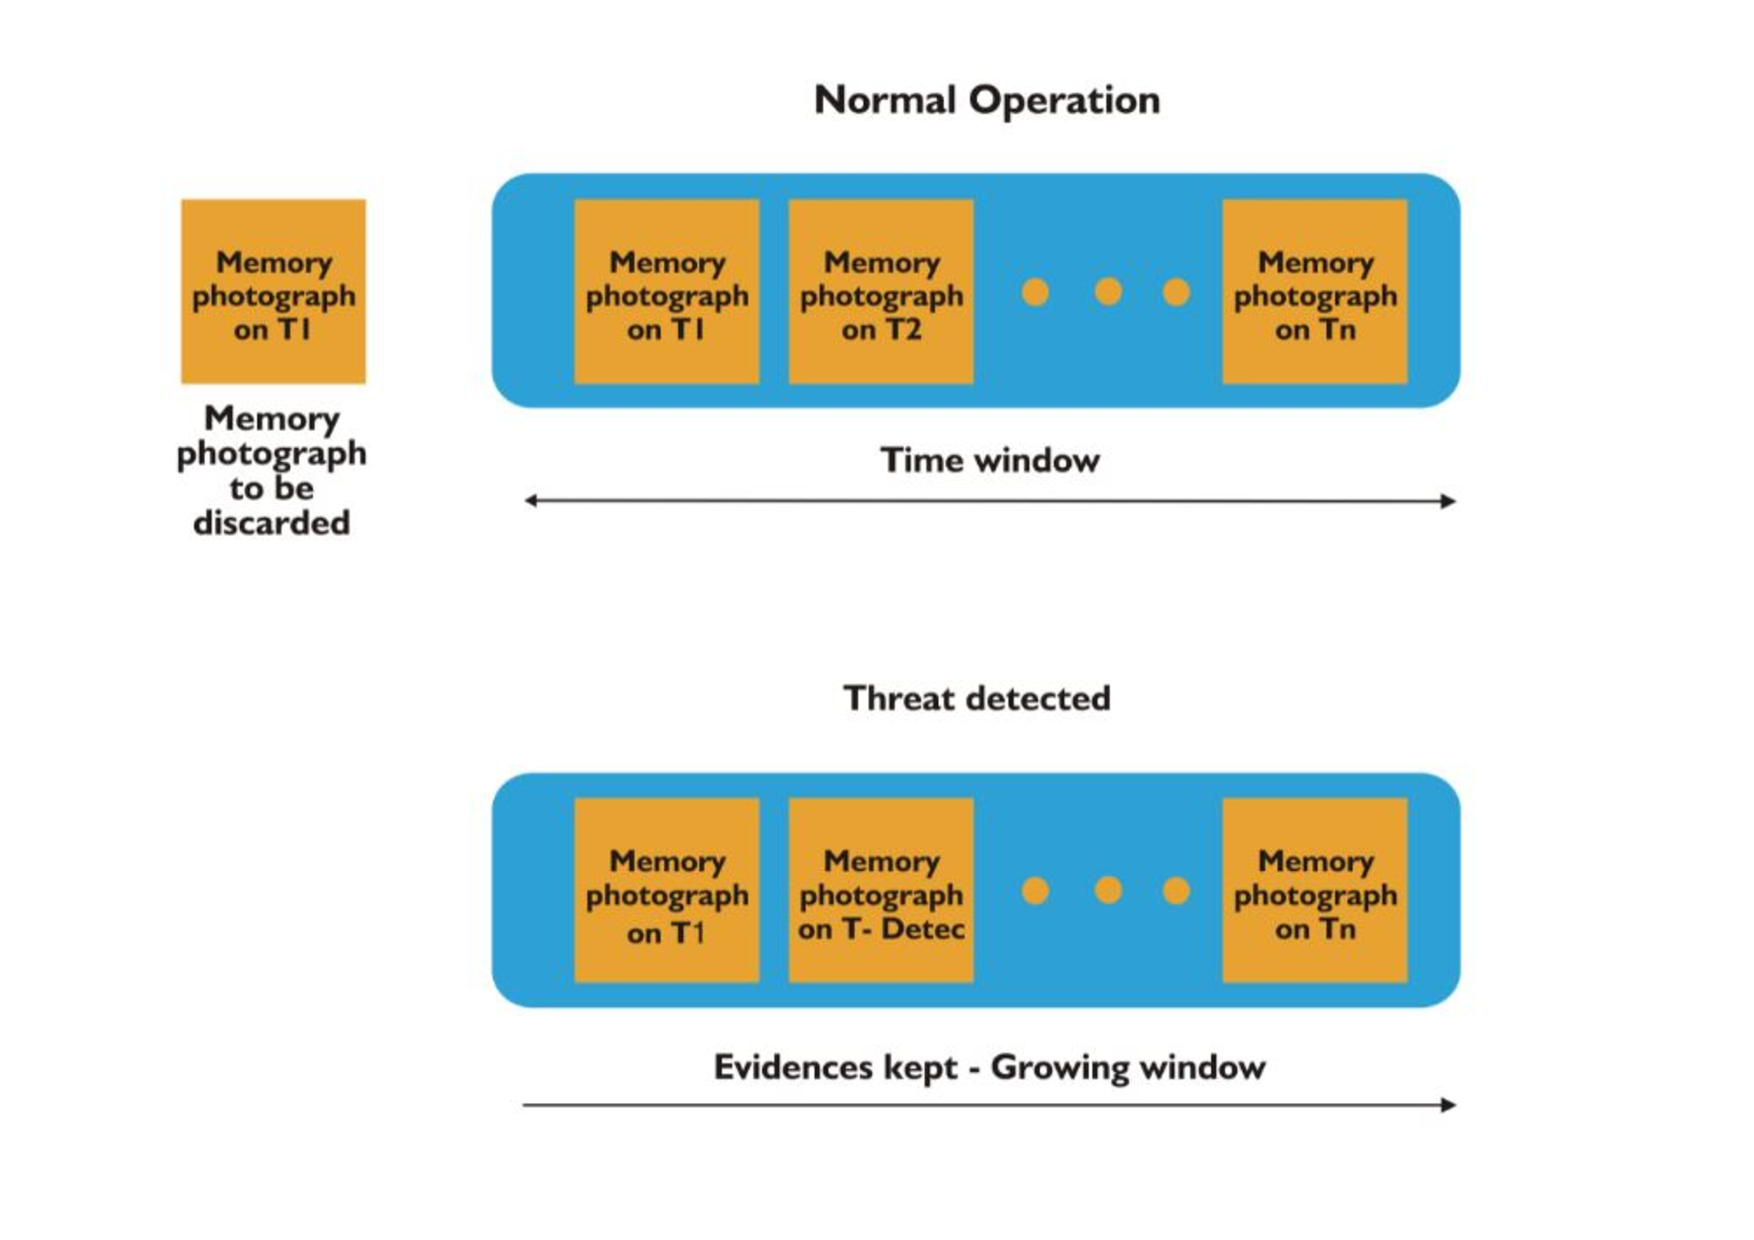
\includegraphics[center,scale=0.70]{janela_ieee-eng.pdf}
    %\centering
    \label{fig:janela}
    \end{figure}
      
    \begin{figure}[h!]
    %\footnotesize
    \caption{\csentence{High level schema} \fancyname's inner working for a single container. }
    %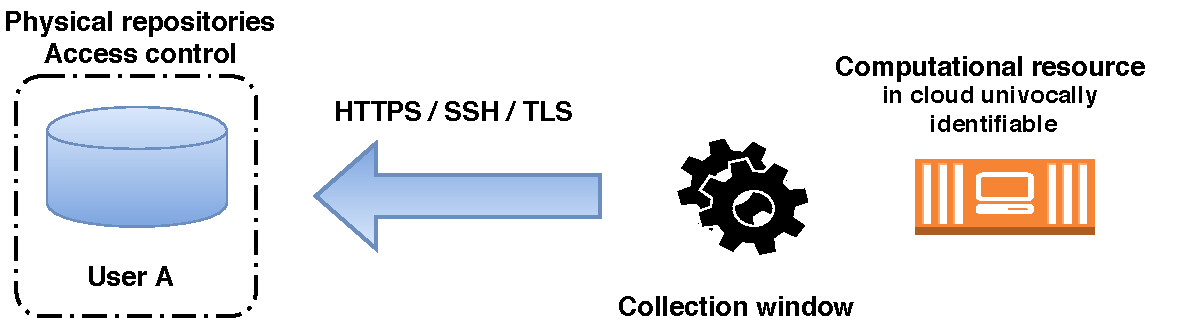
\includegraphics[center,scale=0.45]{solucao-eng-small.pdf}
    %\centering
    \label{fig:Solucao}
    \end{figure}
	  
    \begin{figure}[h!]
    %\footnotesize
    \caption{\csentence{Disk space usage} Evolution of disk space usage while running \fancyname.  }
    %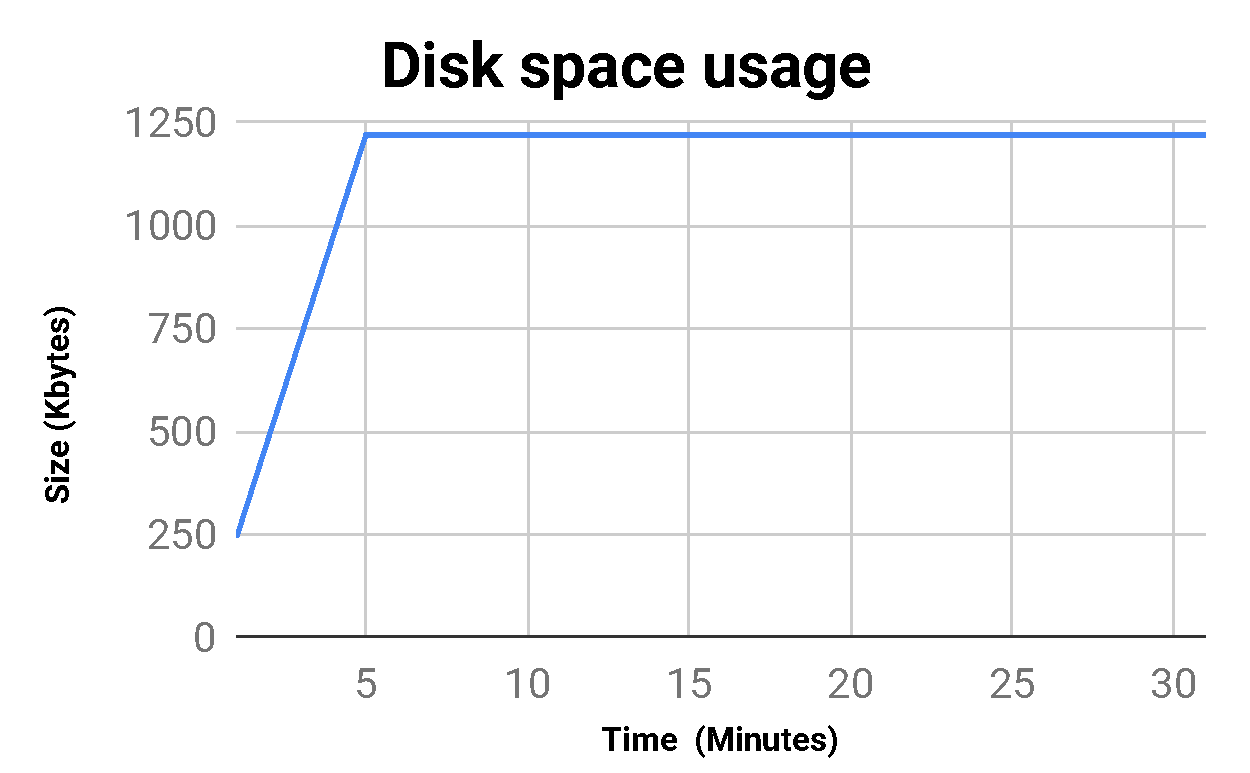
\includegraphics[center,scale=0.40]{evolucao_coleta_ieee.pdf}
    %\centering
    \label{fig:evolucao_coleta}
    \end{figure}
	  
    \begin{figure}[h!]
    %\footnotesize
    \caption{\csentence{Memory copy} Average time for saving a container's snapshot. }
    %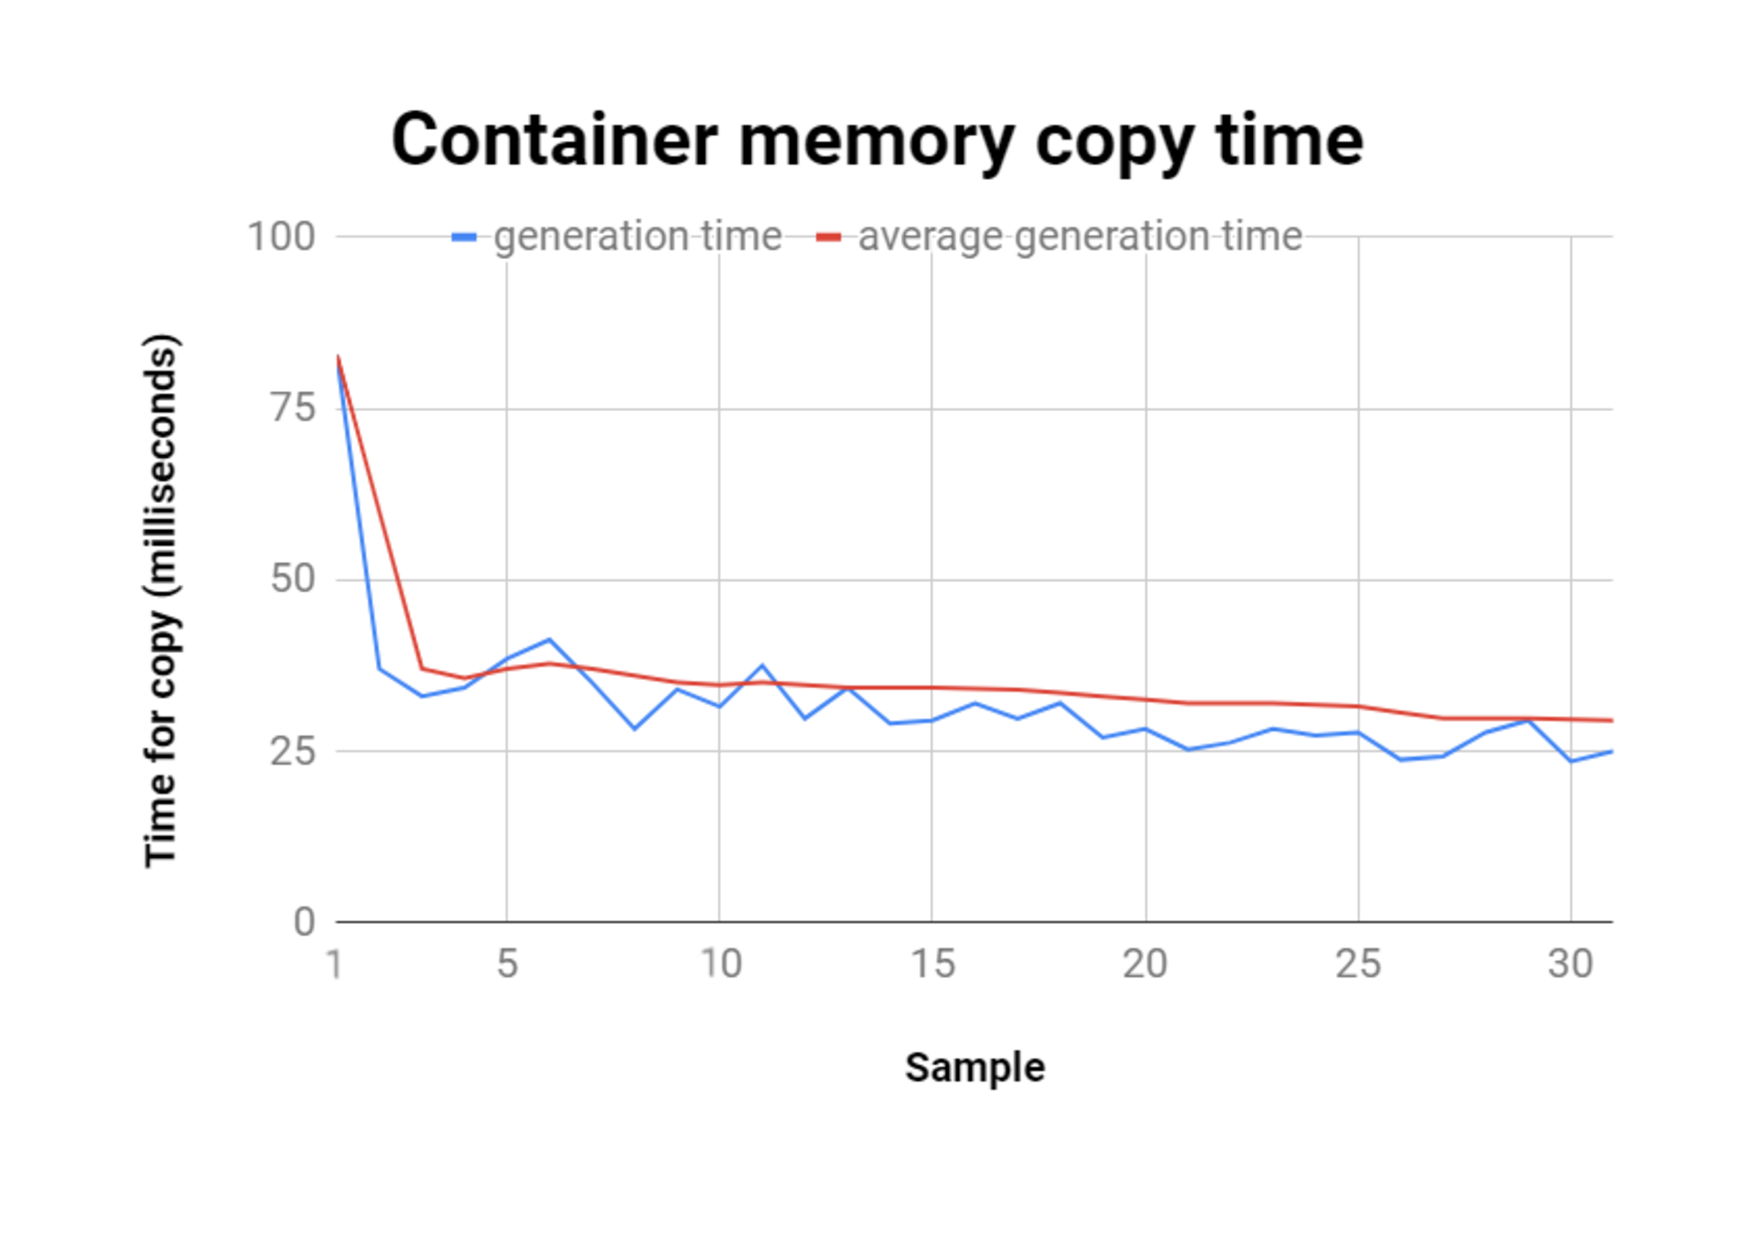
\includegraphics[center,scale=0.45]{memoria_copia_ieee.pdf}
    %\centering
    \label{fig:memoria_copia}
    \end{figure}
	  
    \begin{figure}[htb!]
    %\footnotesize
    \caption{\csentence{Evidence transport time} Average time required for transporting evidences from the cloud to an external storage site. }
    %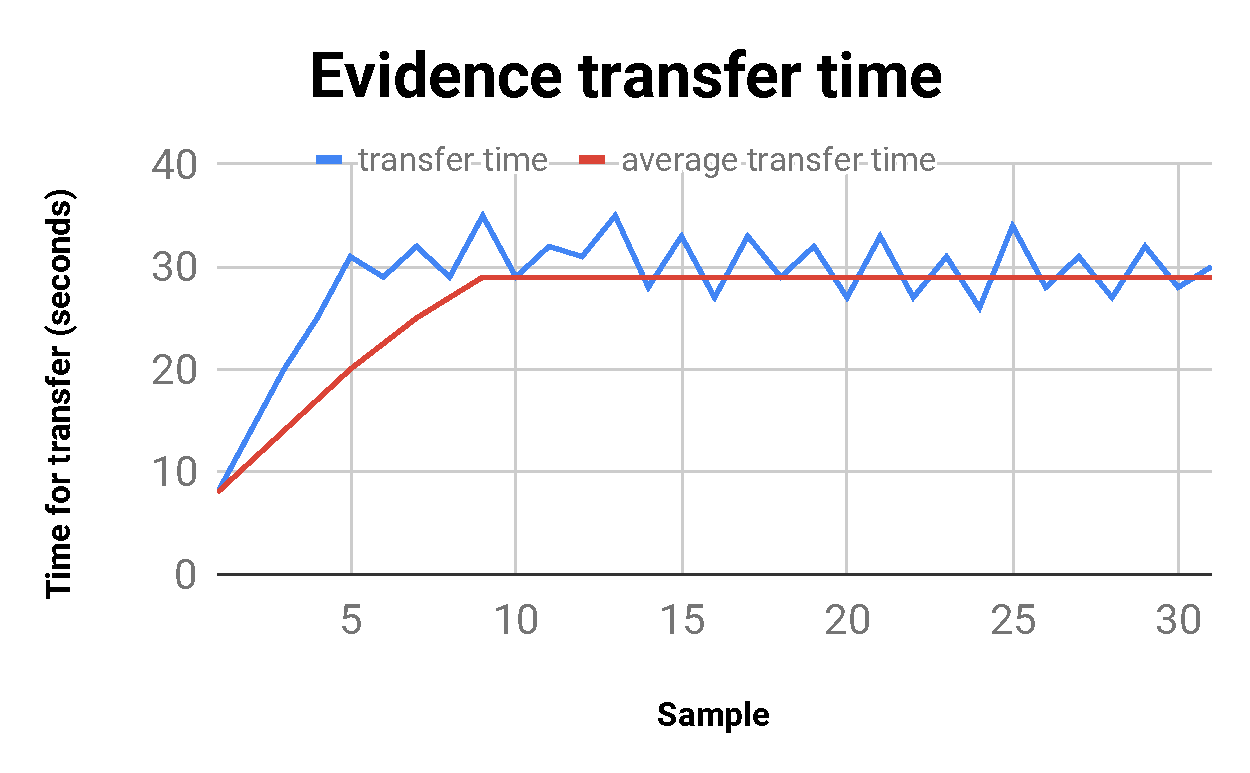
\includegraphics[center,scale=0.45]{evidencia_download_ieee.pdf}
    %\centering
    \label{fig:evidencia_transporte}
    \end{figure}
	  
    \begin{figure}[h!]
    %\footnotesize
    \caption{\csentence{GDB Command} Commands to generate a raw copy of a container's memory. }
    %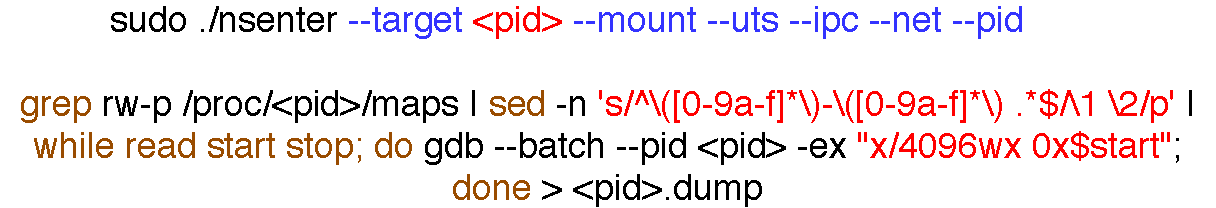
\includegraphics[scale=0.40]{comando-copia-memoria-gdb.pdf}
    %\centering
    \label{fig:comando-copia}
    \end{figure}
	  
    \begin{figure}[h!]
    %\footnotesize
    \caption{\csentence{Before injection} Part of \textbf{/proc/pid/numa\_maps} file BEFORE injection. }
    %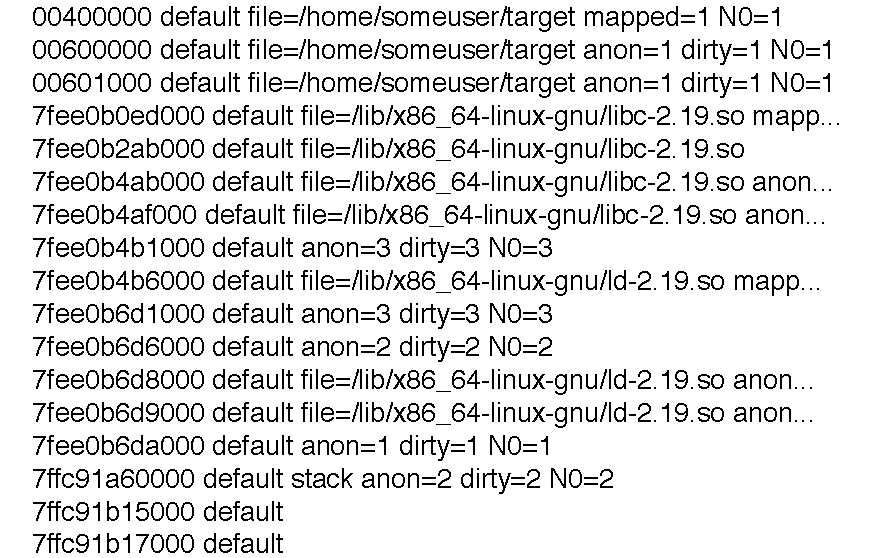
\includegraphics[scale=0.60]{antes-injecao.pdf}
    %\centering
    \label{fig:antes-injecao}
    \end{figure}

    \begin{figure}[h!]
    %\footnotesize
    \caption{\csentence{After injection} Part of \textbf{/proc/pid/numa\_maps} file AFTER injection. }
    %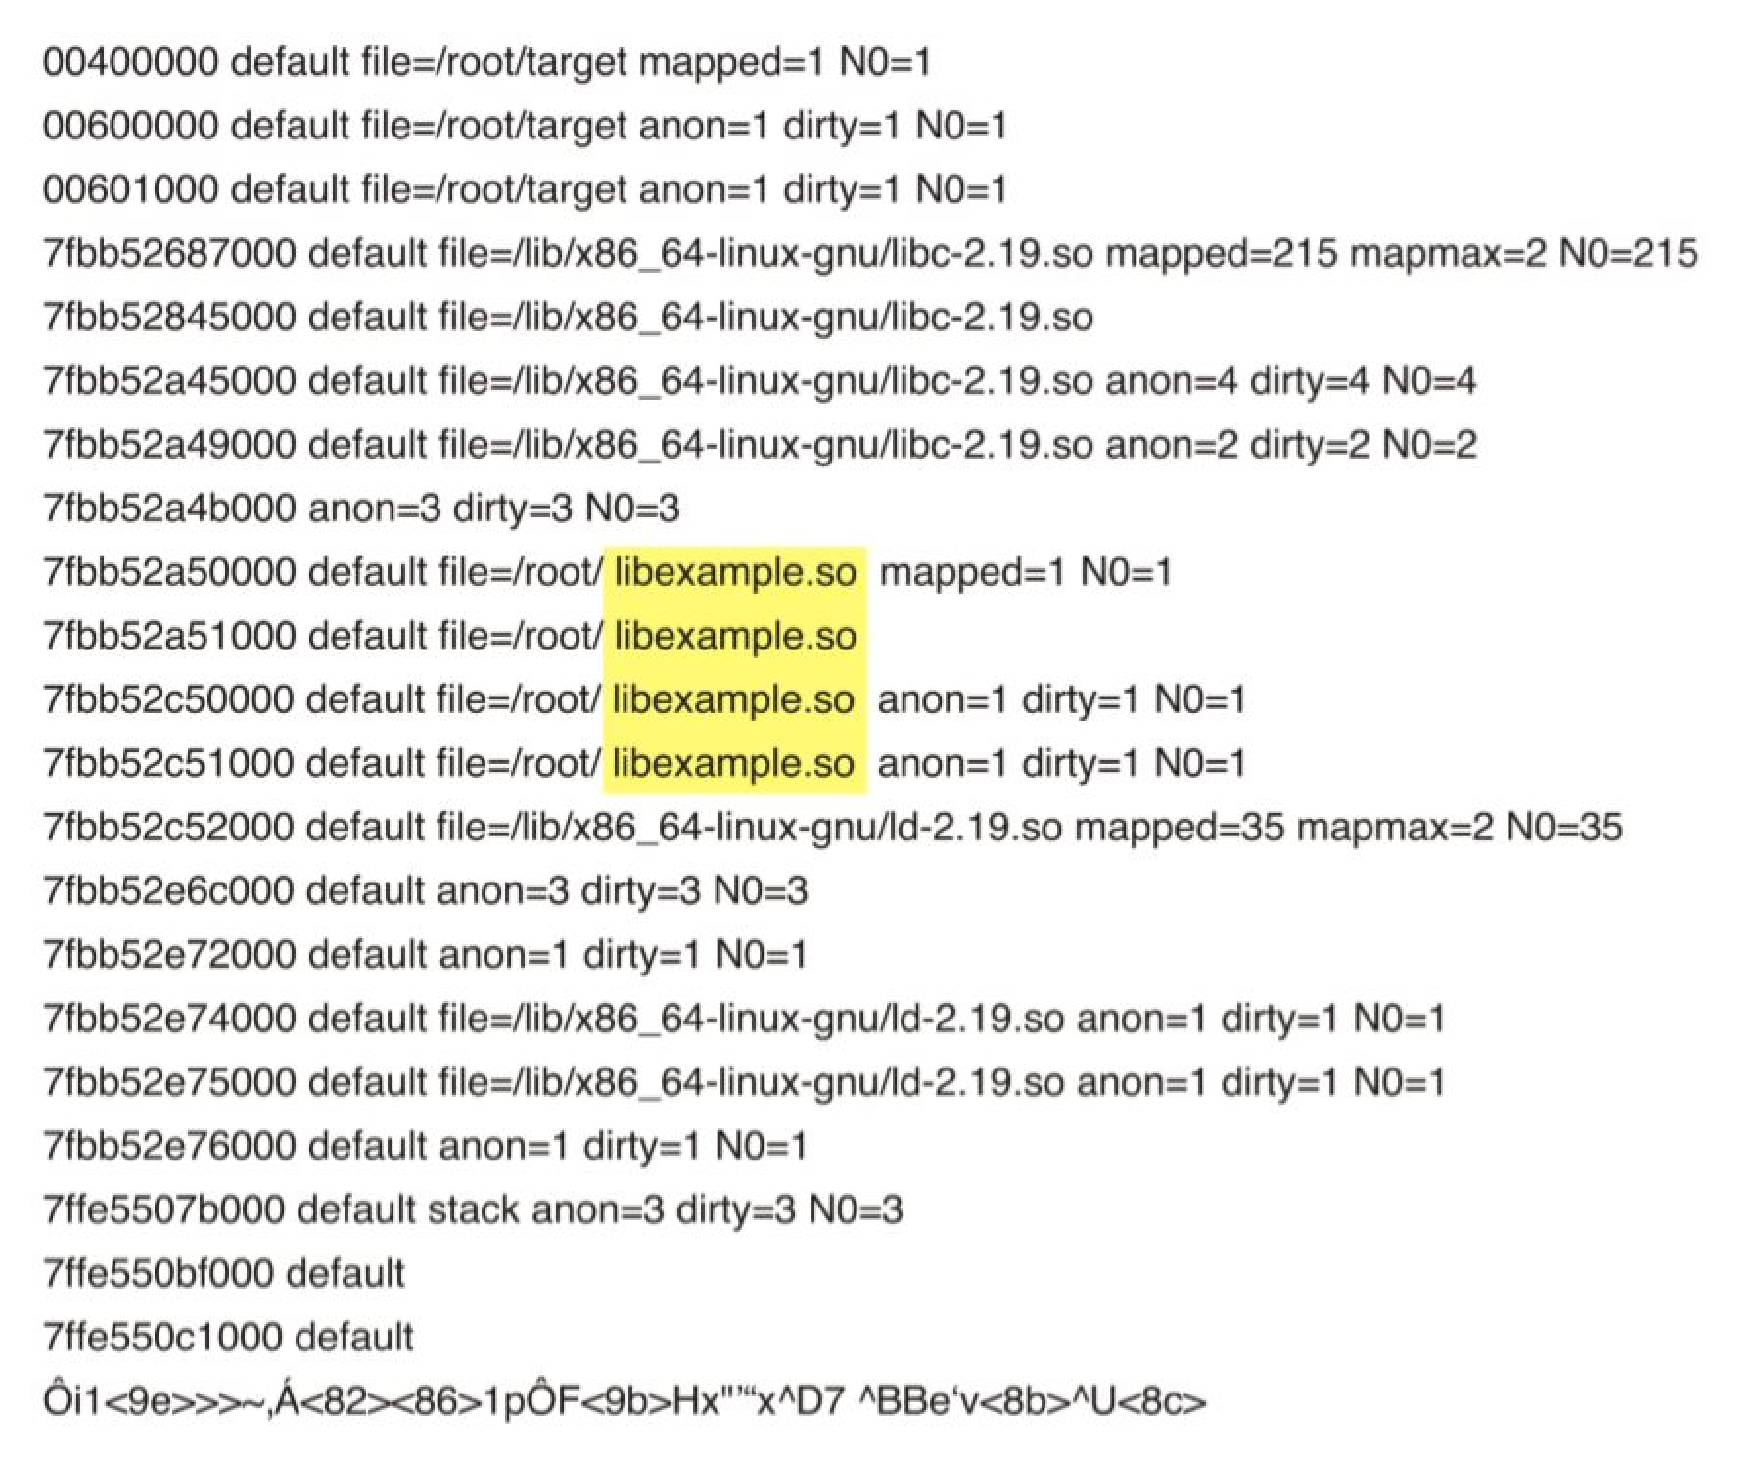
\includegraphics[center,scale=0.60]{apos-injecao.pdf}
    %\centering
    \label{fig:apos-injecao}
    \end{figure}
	
    \begin{figure}[h!]
    %\footnotesize
    \caption{\csentence{Raw memory} Sample of the library's memory inside the container. }
    %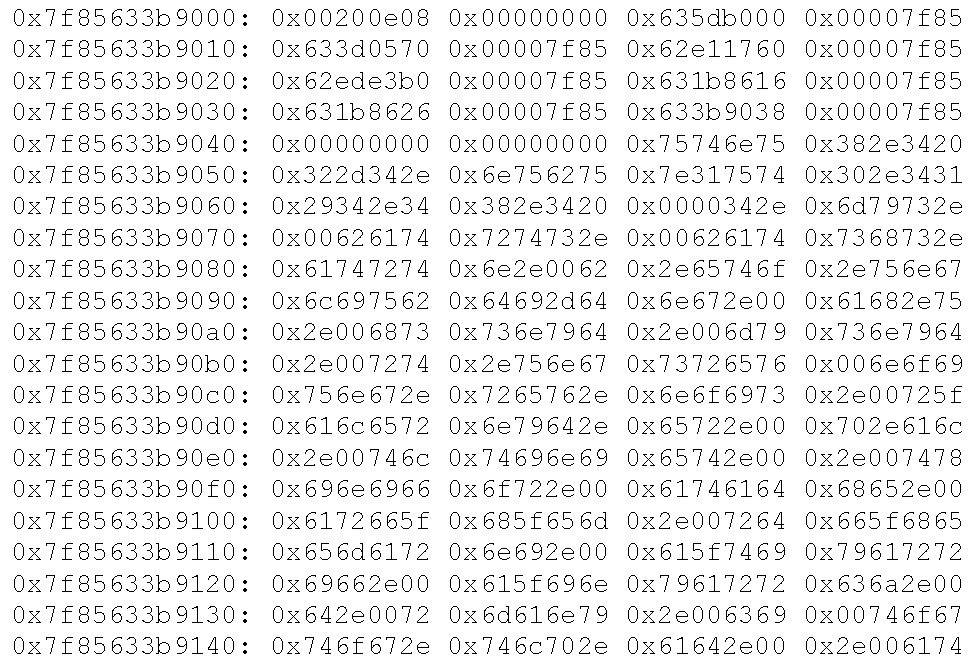
\includegraphics[scale=0.54]{conteudo-memoria-copia-gdb.pdf}
    %\centering
    \label{fig:conteudo-memoria-copia-gdb}
    \end{figure}


%%%%%%%%%%%%%%%%%%%%%%%%%%%%%%%%%%%
%%                               %%
%% Tables                        %%
%%                               %%
%%%%%%%%%%%%%%%%%%%%%%%%%%%%%%%%%%%

%% Use of \listoftables is discouraged.
%%


\section*{Tables}

\begin{table}[h!]
\centering
\caption{Solutions for collecting memory information from cloud machines for forensic analysis}
\label{tab:related-work}
\renewcommand{\arraystretch}{2}
\begin{tabular}{p{3.0cm}|L|L|L|L|}
\cline{2-5}
\textbf{}															& \rotb{Continuous collection \\ of relevant data}	
																											& \rotb{Chain of custody \\ guarantees}
																																		& \rotb{Ability to reproduce \\ the evidence collection \\ process} 
																																									& \rotb{Jurisdiction and \\ privacy preservation}          \\ \hline

\fancyname\ (this proposal)						& \cfig	  			& \cfig       & \cfig       & \cfig                             \\ \hline
\cite{George_DF2CE:2012}							& \xfig		  		& \xfig       & \xfig       & \cfig                             \\ \hline
\cite{Poisel_VMI:2013}								& \xfig       	& \xfig       & \xfig       & \cfig                             \\ \hline
\cite{Dykstra_FROST:2013}							& \xfig      		& \xfig       & \xfig       & \cfig                             \\ \hline
%\cite{Do_Desafio:2014}								& \xfig		    	& \xfig       & \xfig       & \cfig                             \\ \hline
\cite{Reichert_Auto_acquisition:2015}	& \xfig  	    	& \cfig       & \xfig       & \cfig                             \\ \hline
\cite{Sang_Log_approach:2013}					& \cfig   			& \cfig	      & \xfig       & \cfig                             \\ \hline
\cite{Dolan-Gavitt_Semantic_Gap:2011}	& \xfig       	& \xfig       & \xfig       & \cfig                             \\ \hline
\cite{Aljaedi_Comparative:2011}				& \xfig       	& \xfig       & \xfig       & \cfig                             \\ \hline
\cite{Dezfouli_Backup_approach:2012}	& \cfig   			& \xfig       & \xfig       & \cfig                             \\ \hline
\cite{VanBaar_FAAS:2014}							& \cfig   			& \cfig       & \xfig       & \cfig                             \\\hline
\end{tabular}
\end{table}

\end{backmatter}
\end{document}
